\documentclass[11pt,letterpaper]{article}

% Required Packages
\usepackage[utf8]{inputenc}
\usepackage{amsmath}
\usepackage{amsfonts}
\usepackage{amssymb}
\usepackage{graphicx}
\usepackage{geometry}
\usepackage{fancyhdr}
\usepackage{enumitem}
\usepackage{booktabs}
\usepackage{array}
\usepackage{multirow}
\usepackage{xcolor}
\usepackage{hyperref}
\usepackage{listings}
\usepackage{tikz}
\usepackage{pgfplots}
\pgfplotsset{compat=1.18}

% Custom Commands
\newcommand{\milestone}[1]{\textbf{\textcolor{blue}{#1}}}
\newcommand{\metric}[1]{\textbf{\textcolor{green}{#1}}}
\newcommand{\risk}[1]{\textbf{\textcolor{red}{#1}}}
\newcommand{\mitigation}[1]{\textbf{\textcolor{orange}{#1}}}
\newcommand{\techterm}[1]{\textbf{\textcolor{purple}{#1}}}
\newcommand{\code}[1]{\texttt{\textcolor{blue}{#1}}}

% Document Metadata
\newcommand{\projectname}{Non-Question Proficiency Evaluation Framework}
\newcommand{\projectsubtitle}{Methodology Comparison and Ranking Report}
\newcommand{\authorteam}{Research Analysis Team}
\newcommand{\documentversion}{1.0}
\newcommand{\documentdate}{\today}
\newcommand{\documentstatus}{Final Report}

\geometry{margin=1in}
\pagestyle{fancy}
\fancyhf{}
\lhead{\projectname}
\rhead{\projectsubtitle}
\cfoot{\thepage}

\hypersetup{
  colorlinks=true,
  linkcolor=blue,
  urlcolor=blue,
  citecolor=blue
}

\begin{document}

% =========================
% Title Page
% =========================
\begin{titlepage}
\centering
\vspace*{1.2in}
{\LARGE \textbf{\projectname}}\\[0.25in]
{\Large \projectsubtitle}\\[0.6in]
\begin{tabular}{rl}
\textbf{Author Team:} & \authorteam \\
\textbf{Version:} & \documentversion \\
\textbf{Date:} & \documentdate \\
\textbf{Status:} & \documentstatus \\
\end{tabular}
\vfill
\end{titlepage}

\tableofcontents
\newpage

% =========================
% Executive Summary
% =========================
\section{Executive Summary}

This report answers a single decision question: \textit{Which method is best for estimating proficiency gain from non-question learning activities in the \projectname?} All analysis is based \textbf{only} on the provided source material (\textit{Feasibility and Methods.txt}). The source frames the problem as an \techterm{estimation problem under uncertainty}: non-question interactions (watching, reading, simulation use) provide \techterm{rich engagement data} but weaker proof than right/wrong assessment signals. Therefore, a production framework must explicitly represent \techterm{confidence} and treat engagement-driven gains as \textit{lower-confidence evidence} until later validated by an assessment signal.

\subsection{What the evidence supports}
The source provides several empirical anchors:
\begin{itemize}[leftmargin=1.2em]
  \item Engagement measures such as time spent, completion, and re-engagement correlate with better outcomes; reported correlations fall in a moderate-to-strong range (\metric{r = 0.40 to 0.65}).
  \item For video, fine-grained behaviors matter: \textit{pausing and rewinding} correlate positively with exam performance, while frequent fast-forwarding correlates negatively.
  \item For interactive/game-like content, Pearson's \techterm{SPRING} pipeline predicted test outcomes from game logs with correlation around \metric{0.55}, demonstrating feasibility without direct questions.
  \item Duolingo's \techterm{Half-Life Regression (HLR)} improved word recall prediction and increased daily retention by \metric{12\%} (as reported in the source).
  \item Major platforms generally collect engagement data but remain conservative about treating it as proof of mastery (e.g., mastery systems remain assessment-centric; engagement is used to support, intervene, or recommend content).
\end{itemize}

\subsection{Top-ranked methods and the bottom line}
A strict ranking is useful, but the source implies a practical truth: \textbf{no single method dominates across all content types} because the available evidence differs (video clickstream vs. interactive action sequences vs. reading traces). As a result, the best system is \textbf{tiered} and \textbf{content-aware}:
\begin{itemize}[leftmargin=1.2em]
  \item \textbf{Interactive content:} \techterm{Stealth Assessment (SPRING-style)} is the strongest fit when game/action logs exist.
  \item \textbf{Spaced practice / memory-like skills:} \techterm{HLR} is the most defensible where forgetting and recall over time are central.
  \item \textbf{General-purpose skill-state estimation from engagement:} \techterm{EW-BKT} is the best ``backbone'' because it directly treats content interactions as learning opportunities and updates a probabilistic skill state using engagement signals.
\end{itemize}

\subsection{Recommendations by content type (decision-ready)}
\begin{itemize}[leftmargin=1.2em]
  \item \textbf{Video}: \textbf{CLPM + Time-on-Task/Completion} (and MMAE only if you have multi-signal telemetry and the engineering budget).
  \item \textbf{Text/PDF}: \textbf{Time-on-Task/Completion + TWCM} as a baseline; add \textbf{EW-BKT} once you can map content units to target skills and validate later.
  \item \textbf{Interactive}: \textbf{SPRING-style Stealth Assessment + EW-BKT} (ECD evidence model feeding a probabilistic skill-state layer).
\end{itemize}

\subsection{Implementation priorities}
\begin{enumerate}[leftmargin=1.4em]
  \item \milestone{Phase 0 (Instrumentation)}: standardize event logging across content types and define engagement features explicitly.
  \item \milestone{Phase 1 (Baseline)}: Time-on-Task/Completion + TWCM with conservative confidence labeling (``unconfirmed gain'').
  \item \milestone{Phase 2 (Probabilistic Core)}: EW-BKT skill-state layer fed by engagement features; calibrate to later assessments.
  \item \milestone{Phase 3 (High-fidelity per modality)}: SPRING-style stealth assessment for interactive; CLPM and/or MMAE for rich video signals; selective DKT where sequential patterns are predictive and validated.
\end{enumerate}

\newpage

% =========================
% Introduction
% =========================
\section{Introduction}

\subsection{Problem statement}
The \projectname requires estimating learning progress when users consume learning material without answering explicit questions. The source emphasizes that, unlike assessments, these interactions do not provide ``right/wrong'' labels; instead they provide \techterm{engagement traces} that can be interpreted as probabilistic evidence of learning. Because passive study is less predictive of retention than active practice, the system must treat engagement-derived gains as \textbf{lower-confidence} and ideally confirm them later through assessment.

\subsection{Objectives}
This report:
\begin{itemize}[leftmargin=1.2em]
  \item enumerates all \textbf{13 methods} named in the source;
  \item evaluates each method against a fixed criterion set;
  \item ranks the methods using a weighted scoring model;
  \item recommends the best method(s) per content type (video, text/PDF, interactive);
  \item proposes an implementation roadmap consistent with the source's caution about confidence and validation.
\end{itemize}

\subsection{Scope and evidence constraints}
\textbf{Critical constraint:} all claims, method descriptions, and evidence statements are derived only from \textit{Feasibility and Methods.txt}. No external methods, assumptions, datasets, or adoption claims are introduced beyond what is present in that file.

\newpage

% =========================
% Methodology Review
% =========================
\section{Comprehensive Methodology Review}

\subsection{Method inventory (all 13 methods)}
\begin{table}[h]
\centering
\caption{All methods explicitly identified in the source, grouped by category.}
\begin{tabular}{p{4.6in}p{1.3in}}
\toprule
\textbf{Method} & \textbf{Category} \\
\midrule
Heuristic Point Systems (XP Models) & Heuristic \\
Time-on-Task \& Completion Metrics & Heuristic \\
Mastery-Based Engagement Scoring (MBES) & Heuristic \\
Time-Weighted Completion Model (TWCM) & Heuristic \\
Engagement-Weighted Bayesian Knowledge Tracing (EW-BKT) & Model-Based \\
Half-Life Regression (HLR) & Model-Based \\
Performance Factors Analysis (PFA) with Engagement Covariates & Model-Based \\
Item Response Theory (IRT) Analogy & Model-Based \\
Cognitive Load Proxy Model (CLPM) & Model-Based \\
Deep Knowledge Tracing (DKT) with Engagement Features & ML-Based \\
Stealth Assessment (e.g., Pearson's SPRING) & ML-Based \\
Multi-Modal Attention Models (MMAE) & ML-Based \\
Regression/Classification Predictive Models & ML-Based \\
\\\bottomrule
\end{tabular}
\end{table}

\subsection{Heuristic-based methods}
Heuristic approaches provide immediate, interpretable signals (often for gamification or progress feedback). The source positions them as rule-based and not statistical inference.

\subsubsection{Heuristic Point Systems (XP Models)}
\textbf{Definition (from source):} assign experience points or progress percentages for completing content.\\
\textbf{Role:} gamification and immediate feedback.\\
\textbf{Key limitation (from source framing):} XP is not treated as definitive mastery evidence; major platforms are conservative about equating content consumption to proficiency.

\subsubsection{Time-on-Task \& Completion Metrics}
\textbf{Definition (from source):} use normalized time spent and completion rates (e.g., percentage of video watched) as direct predictors.\\
\textbf{Evidence connection:} the source reports consistent correlations between engagement (time/completion) and outcomes, and highlights video behaviors (pause/rewind vs. fast-forward) as informative.

\subsubsection{Mastery-Based Engagement Scoring (MBES)}
\textbf{Definition (from source):} threshold-based levels (Attempted, Familiar, Proficient, Mastered) assigned from engagement triggers.\\
\textbf{Interpretation:} a discrete staging system for progress, likely requiring conservative labeling to avoid overstating proficiency.

\subsubsection{Time-Weighted Completion Model (TWCM)}
\textbf{Definition (from source):} weight completion by quality of time spent relative to expected duration.\\
\textbf{Interpretation:} a simple adjustment to completion that penalizes overly fast skimming and can be used as a baseline.

\subsection{Model-based (probabilistic and statistical) methods}
These approaches incorporate cognitive/psychological structure and typically expose parameters that can be calibrated.

\subsubsection{Engagement-Weighted Bayesian Knowledge Tracing (EW-BKT)}
\textbf{Definition (from source):} extension of BKT treating content interactions as learning opportunities; engagement signals (completion, interaction density) modify the probability a student transitions from unlearned to learned.\\
\textbf{Why it matters:} it directly encodes uncertainty and can label engagement-derived evidence as probabilistic, matching the source's ``uncertainty'' framing.

\subsubsection{Half-Life Regression (HLR)}
\textbf{Definition (from source):} combines the Ebbinghaus forgetting curve with engagement data to estimate memory strength and predict recall probability over time.\\
\textbf{Evidence connection:} the source reports Duolingo's HLR improved prediction and increased daily retention by 12\%.

\subsubsection{Performance Factors Analysis (PFA) with Engagement Covariates}
\textbf{Definition (from source):} logistic regression incorporating prior performance and current engagement to predict proficiency.\\
\textbf{Note:} requires performance history; engagement alone is a covariate.

\subsubsection{Item Response Theory (IRT) Analogy}
\textbf{Definition (from source):} adapt IRT by treating content pieces as ``items'' with difficulty, validated by future success on related questions.\\
\textbf{Implication:} by design, it expects later assessments to confirm engagement-derived gains.

\subsubsection{Cognitive Load Proxy Model (CLPM)}
\textbf{Definition (from source):} estimate productive (germane) vs extraneous load from engagement patterns such as pauses and rewinds.\\
\textbf{Evidence connection:} the source specifically identifies pause/rewind behaviors as predictive signals in video contexts.

\subsection{Machine learning methods}
These methods learn complex mappings from logs to outcomes, typically requiring labeled outcomes for training and strong validation practice.

\subsubsection{Deep Knowledge Tracing (DKT) with Engagement Features}
\textbf{Definition (from source):} uses RNNs or Transformers to process sequences of interactions (including non-question data) to predict future performance.\\
\textbf{Implication:} high expressiveness, but higher complexity and heavier validation requirements.

\subsubsection{Stealth Assessment (SPRING-style)}
\textbf{Definition (from source):} data-driven pipeline using Evidence-Centered Design (ECD) to infer proficiency from action sequences and game logs without direct questions.\\
\textbf{Evidence connection:} the source reports SPRING predicted test outcomes from game logs with correlation $\approx 0.55$.

\subsubsection{Multi-Modal Attention Models (MMAE)}
\textbf{Definition (from source):} combine signals such as scroll depth, video playback speed changes, and session frequency to infer attention quality and learning.\\
\textbf{Implication:} potentially strong where multi-signal telemetry exists, but likely complex and calibration-heavy.

\subsubsection{Regression/Classification Predictive Models}
\textbf{Definition (from source):} direct models (e.g., Random Forests, Logistic Regression) trained to predict final exam scores or mastery states early using clickstream features.\\
\textbf{Evidence connection:} the source notes MOOC research where early attendance/utilization predict eventual passing and that engagement metrics can drive early intervention.

\newpage

% =========================
% Ranking and Evaluation
% =========================
\section{Systematic Ranking and Evaluation}

\subsection{Evaluation criteria and weights}
Weights are chosen to reflect the source's emphasis on (a) empirical defensibility, (b) predictive correlation, and (c) practical deployability under uncertainty.

\begin{table}[h]
\centering
\caption{Evaluation criteria weights (sum to 1.00).}
\begin{tabular}{p{4.8in}r}
\toprule
\textbf{Criterion} & \textbf{Weight} \\
\midrule
Empirical Validity & 0.20 \\
Accuracy and Predictive Power & 0.20 \\
Theoretical Foundation & 0.15 \\
Practical Applicability & 0.15 \\
Generalizability & 0.10 \\
Validation and Calibration & 0.10 \\
Industry Adoption & 0.10 \\
\\\bottomrule
\end{tabular}
\end{table}

\subsection{Scoring rubric (1--5)}
Scores use a 1--5 scale:
\begin{itemize}[leftmargin=1.2em]
\item 1 = weak or unsupported in the source; primarily heuristic or gamification signal
\item 3 = moderate support or plausible fit under the source framing; requires conservative confidence
\item 5 = strong evidence or strong alignment with the source's uncertainty + validation framing
\end{itemize}

\subsection{Full scoring matrix}
\begin{table}[p]
\centering
\small
\caption{Criterion-by-criterion scores for all 13 methods (1--5).}
\begin{tabular}{p{2.55in}ccccccc r}
\toprule
\textbf{Method} & \rotatebox{90}{Emp} & \rotatebox{90}{Acc} & \rotatebox{90}{Theory} & \rotatebox{90}{Prac} & \rotatebox{90}{Gen} & \rotatebox{90}{Val} & \rotatebox{90}{Adopt} & \textbf{Weighted} \\
\midrule
Heuristic Point Systems (XP Models) & 1 & 1 & 1 & 5 & 3 & 1 & 4 & 2.10 \\
Time-on-Task \& Completion Metrics & 3 & 2 & 2 & 5 & 4 & 2 & 4 & 3.05 \\
Mastery-Based Engagement Scoring (MBES) & 1 & 2 & 2 & 4 & 3 & 1 & 2 & 2.10 \\
Time-Weighted Completion Model (TWCM) & 2 & 2 & 2 & 5 & 3 & 1 & 2 & 2.45 \\
Engagement-Weighted Bayesian Knowledge Tracing (EW-BKT) & 4 & 4 & 5 & 3 & 4 & 4 & 2 & 3.80 \\
Half-Life Regression (HLR) & 4 & 4 & 5 & 4 & 3 & 4 & 4 & 4.05 \\
Performance Factors Analysis (PFA) with Engagement Covariates & 3 & 3 & 4 & 3 & 3 & 3 & 1 & 2.95 \\
Item Response Theory (IRT) Analogy & 2 & 2 & 4 & 2 & 3 & 3 & 1 & 2.40 \\
Cognitive Load Proxy Model (CLPM) & 3 & 3 & 4 & 3 & 3 & 2 & 1 & 2.85 \\
Deep Knowledge Tracing (DKT) with Engagement Features & 3 & 4 & 4 & 2 & 4 & 3 & 2 & 3.20 \\
Stealth Assessment (e.g., Pearson's SPRING) & 5 & 4 & 5 & 2 & 4 & 5 & 3 & 4.05 \\
Multi-Modal Attention Models (MMAE) & 2 & 3 & 3 & 2 & 4 & 2 & 1 & 2.45 \\
Regression/Classification Predictive Models & 3 & 3 & 3 & 4 & 4 & 3 & 3 & 3.25 \\
\\\bottomrule
\end{tabular}
\end{table}

\subsection{Overall ranking and tiers}
\begin{table}[h]
\centering
\caption{Overall ranking by weighted score.}
\begin{tabular}{r p{4.4in} r l}
\toprule
\textbf{Rank} & \textbf{Method} & \textbf{Score} & \textbf{Tier} \\
\midrule
1 & Half-Life Regression (HLR) & 4.05 & Tier 1 \\
2 & Stealth Assessment (e.g., Pearson's SPRING) & 4.05 & Tier 1 \\
3 & Engagement-Weighted Bayesian Knowledge Tracing (EW-BKT) & 3.80 & Tier 1 \\
4 & Regression/Classification Predictive Models & 3.25 & Tier 2 \\
5 & Deep Knowledge Tracing (DKT) with Engagement Features & 3.20 & Tier 2 \\
6 & Time-on-Task \& Completion Metrics & 3.05 & Tier 2 \\
7 & Performance Factors Analysis (PFA) with Engagement Covariates & 2.95 & Tier 3 \\
8 & Cognitive Load Proxy Model (CLPM) & 2.85 & Tier 3 \\
9 & Time-Weighted Completion Model (TWCM) & 2.45 & Tier 3 \\
10 & Multi-Modal Attention Models (MMAE) & 2.45 & Tier 3 \\
11 & Item Response Theory (IRT) Analogy & 2.40 & Tier 3 \\
12 & Heuristic Point Systems (XP Models) & 2.10 & Tier 4 \\
13 & Mastery-Based Engagement Scoring (MBES) & 2.10 & Tier 4 \\
\\\bottomrule
\end{tabular}
\end{table}

\subsection{Ranking visualization}
\begin{figure}[h]
\centering
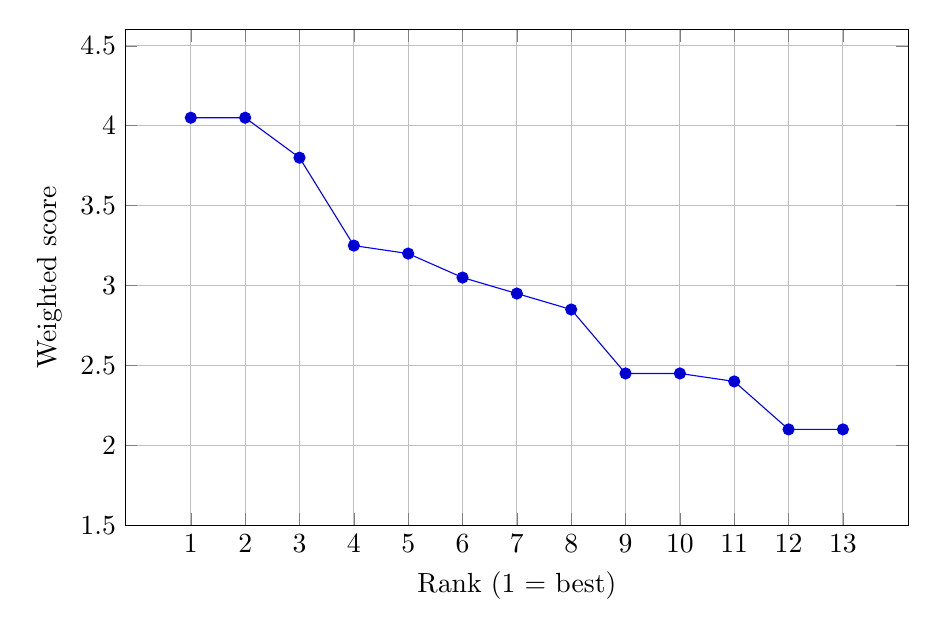
\begin{tikzpicture}
\begin{axis}[
  width=0.95\textwidth,
  height=3.1in,
  xlabel={Rank (1 = best)},
  ylabel={Weighted score},
  ymin=1.5, ymax=4.6,
  xtick={1,2,3,4,5,6,7,8,9,10,11,12,13},
  grid=both
]
\addplot coordinates {
(1,4.05)
(2,4.05)
(3,3.80)
(4,3.25)
(5,3.20)
(6,3.05)
(7,2.95)
(8,2.85)
(9,2.45)
(10,2.45)
(11,2.40)
(12,2.10)
(13,2.10)
};
\end{axis}
\end{tikzpicture}
\caption{Weighted scores by rank (higher is better).}
\end{figure}

\subsection{Interpretation of the top tier}
\textbf{Tier 1} methods are the most defensible choices under the source constraints:
\begin{itemize}[leftmargin=1.2em]
  \item \textbf{HLR}: strong theoretical foundation (forgetting curve), reported platform success (retention improvement), and practical deployability where recall over time matters.
  \item \textbf{SPRING-style stealth assessment}: strongest direct evidence for non-question inference from action sequences (reported correlation $\approx 0.55$), especially for interactive content.
  \item \textbf{EW-BKT}: best general-purpose probabilistic skill-state update from content interactions; aligns directly with the ``estimation under uncertainty'' framing.
\end{itemize}

\newpage

% =========================
% Comparative Analysis
% =========================
\section{Comparative Analysis}

\subsection{Strengths and weaknesses (by category)}
\subsubsection{Heuristic methods}
\textbf{Strengths:} simplicity, transparency, fast deployment, immediate feedback.\\
\textbf{Weaknesses:} weak as proof of proficiency; must be labeled as low-confidence and calibrated against assessments.

\subsubsection{Model-based methods}
\textbf{Strengths:} explicit uncertainty; grounded cognitive structure (learning/forgetting); easier to calibrate than deep models.\\
\textbf{Weaknesses:} require design choices (skill mapping, parameter calibration) and, in some cases, performance history.

\subsubsection{ML methods}
\textbf{Strengths:} capture non-linear patterns and sequences; strong potential where rich logs exist (e.g., action sequences, clickstreams).\\
\textbf{Weaknesses:} higher implementation complexity; require careful validation/calibration to avoid overconfident inferences from passive engagement.

\subsection{Side-by-side comparison (practical decision matrix)}
\begin{table}[h]
\centering
\caption{High-level decision matrix (derived from the source framing).}
\begin{tabular}{p{2.2in}p{1.5in}p{1.5in}p{1.5in}}
\toprule
\textbf{Question} & \textbf{Heuristic} & \textbf{Model-based} & \textbf{ML-based} \\
\midrule
Fast to implement? & High & Medium & Low \\
Explicit uncertainty? & Low & High & Medium (depends on calibration) \\
Needs labeled outcomes? & Low & Medium & High \\
Best for early baseline? & Yes & Yes (after baseline) & Only after data maturity \\
Risk of over-claiming mastery? & High if misused & Lower (probabilistic) & High if uncalibrated \\
\bottomrule
\end{tabular}
\end{table}

\subsection{Implementation complexity (qualitative)}
\begin{itemize}[leftmargin=1.2em]
  \item \textbf{Simple:} XP models, Time-on-Task/Completion, MBES, TWCM.
  \item \textbf{Moderate:} EW-BKT, HLR, PFA+covariates, CLPM, basic regression/classification.
  \item \textbf{Complex:} DKT, SPRING-style stealth assessment, MMAE.
\end{itemize}

\newpage

% =========================
% Content-Specific Recommendations
% =========================
\section{Content-Specific Recommendations}

\subsection{Summary table}
\begin{table}[h]
\centering
\caption{Recommended primary methods by content type (with secondary/backbone options).}
\begin{tabular}{p{1.2in}p{5.2in}}
\toprule
\textbf{Content Type} & \textbf{Recommendation} \\
\midrule
Video & Cognitive Load Proxy Model (CLPM) + Time-on-Task \& Completion + (optionally) MMAE \\
Text/PDF & Time-on-Task \& Completion + TWCM (baseline) ; EW-BKT when you can link content to skills \\
Interactive & Stealth Assessment (SPRING-style ECD pipeline) + EW-BKT (skill-state layer) \\
\bottomrule
\end{tabular}
\end{table}

\subsection{Video content}
\textbf{Primary recommendation:} \techterm{Cognitive Load Proxy Model (CLPM)} combined with \techterm{Time-on-Task \& Completion}.\\
\textbf{Rationale (from source):} the source explicitly identifies pause/rewind as positively correlated with exam performance and fast-forward as negatively correlated. CLPM is designed to interpret these patterns as proxies for productive versus extraneous effort. Time-on-Task/Completion provides a robust baseline aligned with reported engagement correlations.

\textbf{Implementation considerations:}
\begin{itemize}[leftmargin=1.2em]
  \item Capture events: play, pause, rewind/seek-back, seek-forward/fast-forward, playback speed changes, completion percentage, rewatch count.
  \item Assign conservative confidence: video-derived gains should be ``unconfirmed'' until later validated.
  \item Optional upgrade: \techterm{MMAE} when you have scroll depth + speed changes + session frequency and you can afford heavier calibration.
\end{itemize}

\subsection{Text/PDF content}
\textbf{Primary recommendation:} \techterm{Time-on-Task \& Completion} plus \techterm{TWCM} as the baseline, with \techterm{EW-BKT} as the probabilistic upgrade.\\
\textbf{Rationale (from source):} the source provides broad evidence that time, completion, and re-engagement correlate with outcomes. TWCM directly encodes ``quality of time'' relative to expected duration. EW-BKT is appropriate once the system can treat content interactions as learning opportunities and map content units to skills.

\textbf{Implementation considerations:}
\begin{itemize}[leftmargin=1.2em]
  \item Capture events: scroll depth, active time, section completion, return visits, time between sessions.
  \item Use a conservative proficiency increment (lower-confidence evidence).
  \item Validate later: the source repeatedly emphasizes that engagement is not definitive mastery evidence; use later assessments to calibrate.
\end{itemize}

\subsection{Interactive content}
\textbf{Primary recommendation:} \techterm{Stealth Assessment (SPRING-style)} with an \techterm{EW-BKT} skill-state layer.\\
\textbf{Rationale (from source):} the strongest non-question evidence in the source is the SPRING result (correlation $\approx 0.55$) from action sequences and game logs. This is precisely the interactive setting. EW-BKT complements this by maintaining an explicit probabilistic skill state updated by evidence from interactions.

\textbf{Implementation considerations:}
\begin{itemize}[leftmargin=1.2em]
  \item Define evidence model (ECD): which actions support which competencies.
  \item Log action sequences with timestamps and context (levels, attempts, hints, retries).
  \item Calibrate and monitor correlation to external assessments.
\end{itemize}

\newpage

% =========================
% Implementation Roadmap
% =========================
\section{Implementation Roadmap}

\subsection{Phase 0: Instrumentation (mandatory)}
\milestone{Goal:} produce consistent engagement logs across modalities.\\
\metric{Deliverables:}
\begin{itemize}[leftmargin=1.2em]
  \item Unified event taxonomy (video, text/PDF, interactive).
  \item Feature definitions aligned with the source signals (time, completion, re-engagement, pause/rewind/fast-forward, action sequences).
  \item ``Confidence'' labeling policy: engagement-derived gains are lower-confidence until validated.
\end{itemize}

\subsection{Phase 1: Baseline inference (low risk)}
\milestone{Methods:} Time-on-Task/Completion + TWCM, optionally MBES for user-facing progress.\\
\risk{Risk:} over-claiming mastery from passive engagement.\\
\mitigation{Mitigation:} label as ``unconfirmed'' and cap credit per content unit.

\subsection{Phase 2: Probabilistic skill-state core}
\milestone{Methods:} EW-BKT (and HLR where forgetting/recall dynamics dominate).\\
\metric{Deliverables:}
\begin{itemize}[leftmargin=1.2em]
  \item Skill mapping between content units and latent competencies.
  \item Calibration pipeline against assessment outcomes (later quizzes/tests).
\end{itemize}

\subsection{Phase 3: Modality-optimized advanced models}
\milestone{Methods:} SPRING-style stealth assessment for interactive; CLPM and/or MMAE for video; selective DKT for sequence-heavy learning.\\
\risk{Risk:} complex models can be confidently wrong if not validated.\\
\mitigation{Mitigation:} rigorous holdout evaluation against assessment outcomes; conservative confidence and monitoring.

\newpage

% =========================
% Limitations and Future Research
% =========================
\section{Limitations and Future Research}

\subsection{Limitations (as implied by the source)}
\begin{itemize}[leftmargin=1.2em]
  \item Engagement-based estimates are inherently uncertain and should be treated as lower-confidence evidence until validated.
  \item Passive study signals can be weaker indicators of retention than active practice, so over-crediting content consumption is a systematic risk.
  \item Some approaches (e.g., IRT analogy) explicitly depend on later assessment to validate content-derived gains.
  \item Higher-complexity ML methods require strong validation and calibration to remain defensible.
\end{itemize}

\subsection{Future research directions (bounded to the source)}
\begin{itemize}[leftmargin=1.2em]
  \item Improve calibration between engagement metrics and later assessments to move signals from ``unconfirmed'' to confirmed mastery.
  \item Extend cognitive load proxies and multi-modal attention signals where video telemetry supports them.
  \item Evaluate sequential models (DKT) only when there is sufficient outcome data to validate predictive power within the reported correlation band (r = 0.40 to 0.65).
\end{itemize}

\newpage

% =========================
% Conclusion
% =========================
\section{Conclusion and Recommendations}

\subsection{Final answer: which method is best?}
Based strictly on the source, the most defensible conclusion is \textbf{conditional}:
\begin{itemize}[leftmargin=1.2em]
  \item \textbf{Best for interactive logs:} \textbf{SPRING-style stealth assessment} (direct evidence of non-question inference with correlation $\approx 0.55$).
  \item \textbf{Best for memory/recall dynamics:} \textbf{HLR} (reported platform success including 12\% daily retention improvement).
  \item \textbf{Best general-purpose backbone:} \textbf{EW-BKT} (explicitly models content interactions as learning opportunities and updates a probabilistic skill state using engagement signals).
\end{itemize}

\subsection{Non-negotiable design principle}
The system should treat engagement-derived proficiency as \textbf{probabilistic and lower-confidence} until later assessment validates it, exactly as emphasized in the source.

\newpage

% =========================
% References (only those explicitly listed in the source)
% =========================
\begin{thebibliography}{99}

\bibitem{corbett1994}
Corbett, A. T., \& Anderson, J. R. (1994). \textit{Knowledge tracing: Modeling the acquisition of procedural knowledge.}

\bibitem{settles2016}
Settles, B., \& Meeder, B. (2016). \textit{A trainable spaced repetition model.}

\bibitem{gonzalez2016}
Gonzalez-Brenes, et al. (2016). \textit{A Data-Driven Approach for Inferring Student Proficiency from Game Activity Logs.}

\bibitem{piech2015}
Piech, C., et al. (2015). \textit{Deep knowledge tracing.}

\bibitem{guo2014}
Guo, P. J., Kim, J., \& Rubin, R. (2014). \textit{How video production affects student engagement.}

\bibitem{yurum2022}
Yürüm, et al. (2022). \textit{The use of video clickstream data to predict university students’ test performance.}

\bibitem{tong2025}
Tong \& Ren (2025). \textit{Deep knowledge tracing and cognitive load estimation for personalized learning path.}

\bibitem{chi2014}
Chi, M. T. H., \& Wylie, R. (2014). \textit{The ICAP framework: Linking cognitive engagement to active learning outcomes.}

\end{thebibliography}

\end{document}
